%% TeXora template: Accessible Lecture. High-contrast 16:9 slides that show, slide by slide, how to
%% make still content usable with a screen reader: alt text, decoration, described drawings, tables,
%% links, maths and the document language.
%%
%% What it uses:
%%   - accessgate (comes with TeXora; for another editor, keep accessgate.sty beside this file).
%%   - The picture media/test-card.png, which comes with this template.
%%   - Any engine. Tools > Check accessibility lists what is still missing; Build tagged copy
%%     makes a tagged copy (Beamer slides go through the ltx-talk class of TeX Live 2026).
%%
%% Techniques, one per slide:
%%   alt={...} on pictures, artifact for decoration, \AccFigure for drawings, a header rule in tables,
%%   link text that says where it goes, a title on every slide, the language in babel and pdflang.
%% Contrast: ink on white is 16:1, the teal accent 5.6:1 (WCAG asks 4.5:1 for text).
%% Change the colours on the \definecolor lines below.
% !TEX program = pdflatex
\documentclass[aspectratio=169]{beamer}
\usetheme{default}
\usepackage[T1]{fontenc}
\usepackage{lmodern}
\usepackage[english]{babel}
\usepackage{booktabs}
\usepackage{tikz}
\usepackage{accessgate}
\definecolor{ink}{RGB}{20,24,31}
\definecolor{teal}{RGB}{0,110,112}
\definecolor{linkteal}{RGB}{0,122,124}
\definecolor{paper}{RGB}{255,255,255}
\definecolor{haze}{RGB}{228,242,241}
% After the colours: with tagging on, hyperref uses them at once.
\hypersetup{pdflang=en-US,pdftitle={Accessible Lecture},colorlinks,urlcolor=linkteal,linkcolor=ink}
\setbeamercolor{normal text}{fg=ink,bg=paper}
\setbeamercolor{structure}{fg=teal}
\setbeamercolor{frametitle}{fg=ink}
\setbeamercolor{title}{fg=ink}
\setbeamercolor{subtitle}{fg=teal}
\setbeamercolor{block title}{bg=teal,fg=white}
\setbeamercolor{block body}{bg=haze,fg=ink}
\setbeamercolor{alerted text}{fg=teal!80!black}
\setbeamertemplate{blocks}[rounded][shadow=false]
\setbeamertemplate{navigation symbols}{}
\setbeamertemplate{itemize items}[square]
\setbeamertemplate{frametitle}{%
  \vskip0.6em\usebeamerfont{frametitle}\usebeamercolor[fg]{frametitle}\insertframetitle\par
  \AccArtifact{\textcolor{teal}{\rule{2.2cm}{2.5pt}}}\par}
\setbeamertemplate{footline}{%
  \hfill\usebeamercolor[fg]{structure}\scriptsize\insertframenumber\,/\,\inserttotalframenumber\hspace*{1.2em}\vskip0.8em}
\setbeameroption{show notes on second screen=right}

\newcommand{\code}[1]{{\small\ttfamily #1}}

\title{Accessible Lecture}
\subtitle{Slides that everyone can follow, also with a screen reader}
\author{Your Name}
\institute{Your Institution}
\date{\today}

\begin{document}

\begin{frame}
  \vfill
  {\Huge\bfseries\inserttitle\par}
  \vspace{0.5em}
  {\large\usebeamercolor[fg]{subtitle}\insertsubtitle\par}
  \vspace{1.6em}
  \insertauthor\quad\textperiodcentered\quad\insertinstitute\quad\textperiodcentered\quad\insertdate
  \vfill
\end{frame}
\note{Every slide here shows one technique and uses it. Tools, Check accessibility should list nothing to fix for this file.}

\begin{frame}{A title on every slide}
  \begin{itemize}
    \item A screen reader jumps from slide to slide by their titles: give each frame one.
    \item The title slide counts as titled: it shows \code{\textbackslash inserttitle} (or \code{\textbackslash titlepage}).
    \item Steps made with \code{\textbackslash pause} keep the slide's title.\pause
    \item This point comes on the second step.
  \end{itemize}
\end{frame}
\note{The check lists any frame without a title, in every form: begin frame, the frame command and your own frame environments.}

\begin{frame}{Describe every picture}
  \begin{columns}[c]
    \begin{column}{0.42\textwidth}
      \centering
      \includegraphics[width=\linewidth,alt={A television test card: eight vertical colour bars, a rainbow strip and a frame counter}]{media/test-card.png}
    \end{column}
    \begin{column}{0.54\textwidth}
      \code{\textbackslash includegraphics[width=\textbackslash linewidth,}\\
      \code{\ \ alt=\{A television test card: ...\}]\{media/test-card.png\}}
      \par\medskip
      \begin{itemize}
        \item Say what matters, not ``image of''.
        \item One or two sentences; put details in the text.
        \item A chart: give its finding, \emph{sales doubled}.
      \end{itemize}
    \end{column}
  \end{columns}
\end{frame}
\note{alt text reaches the PDF where the LaTeX kernel knows the key, 2023 and later. Older installations still compile.}

\begin{frame}{Decoration is skipped}
  \begin{itemize}
    \item The teal line under every title is decoration: it is wrapped in \code{\textbackslash AccArtifact\{...\}}, so a screen reader passes over it.
    \item A decorative picture: \code{\textbackslash includegraphics[artifact]\{...\}}.
  \end{itemize}
  \par\medskip
  \centering
  \AccArtifact{
\begin{tikzpicture}
    \foreach \i in {0,...,11} \fill[teal!\the\numexpr 20+6*\i\relax] (\i*0.55,0) circle (0.18);
  \end{tikzpicture}}
\end{frame}
\note{Mark as artifact only what carries no meaning. A logo with the organisation's name is not decoration.}

\begin{frame}{Drawings get a description}
  \begin{columns}[c]
    \begin{column}{0.48\textwidth}
      \centering
      \AccFigure{A flow chart: Write, then Check, then Build; an arrow from Check goes back to Write}{%
      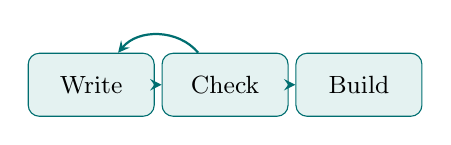
\begin{tikzpicture}[node distance=1.7cm, box/.style={draw=teal,fill=haze,rounded corners,minimum width=1.6cm,minimum height=0.8cm,font=\small}, >=stealth]
        \node[box] (w) {Write};
        \node[box,right of=w] (c) {Check};
        \node[box,right of=c] (b) {Build};
        \draw[->,thick,teal] (w) -- (c);
        \draw[->,thick,teal] (c) -- (b);
        \draw[->,thick,teal] (c) to[bend right=50] (w);
      \end{tikzpicture}}
    \end{column}
    \begin{column}{0.48\textwidth}
      \code{\textbackslash AccFigure\{A flow chart: ...\}\{}\\
      \code{\ \ \textbackslash begin\{tikzpicture\} ...\}}
      \par\medskip
      TikZ, PGFPlots and anything without an \code{alt} key: wrap it in \code{\textbackslash AccFigure}.
    \end{column}
  \end{columns}
\end{frame}

\begin{frame}{Tables with a header row}
  \centering
  \AccHeaderRows{1}
  \begin{tabular}{@{}lll@{}}
    \toprule
    \textbf{Content} & \textbf{What to give it} & \textbf{WCAG} \\
    \midrule
    Picture & \code{alt=\{...\}} or \code{artifact} & 1.1.1 \\
    Video & \code{alt}, and a caption or transcript & 1.2.1 \\
    Animation that loops & a way to pause it & 2.2.2 \\
    Link & text that says where it goes & 2.4.4 \\
    \bottomrule
  \end{tabular}
  \par\medskip
  \small The rule under the first row shows the header row; \code{\textbackslash AccHeaderRows\{1\}} before the table tags it as one.
\end{frame}
\note{Keep tables simple: one header row, no merged cells. A screen reader reads them cell by cell.}

\begin{frame}{Links that say where they go}
  \begin{itemize}
    \item Good: the \href{https://www.w3.org/WAI/WCAG22/quickref/}{WCAG 2.2 quick reference}.
    \item Not: ``click here'' or a bare web address. The check lists those.
    \item Coloured links need 3:1 with the text around them and 4.5:1 with the background (WCAG 1.4.1); the check measures them.
  \end{itemize}
  \par\medskip
  \begin{block}{Maths}
    Write maths as maths, $E = mc^2$ and
    \[ \sum_{k=1}^{n} k = \frac{n(n+1)}{2}, \]
    so the tagged copy keeps it as a formula (with LuaLaTeX also as MathML).
  \end{block}
\end{frame}

\begin{frame}{The language and the title}
  \begin{itemize}
    \item \code{\textbackslash usepackage[english]\{babel\}} and \code{\textbackslash hypersetup\{pdflang=en-US\}}: a screen reader reads with the right voice.
    \item \code{\textbackslash title\{...\}} and \code{pdftitle}: the window shows the title, not the file name.
    \item Colour is never the only signal: the bold header row and the step numbers say the same.
  \end{itemize}
\end{frame}

\begin{frame}{Your turn}
  \begin{enumerate}
    \item Replace the text and the picture with your own; give each picture its \code{alt}.
    \item \textbf{Tools > Check accessibility}: fix what it lists, line by line.
    \item \textbf{Build tagged copy}: \code{talk.acc.pdf}, a tagged copy for screen readers.
  \end{enumerate}
\end{frame}
\note{Thank the audience. The tagged copy leaves this file and its PDF as they are.}

\end{document}
